\PassOptionsToPackage{unicode=true}{hyperref} % options for packages loaded elsewhere
\PassOptionsToPackage{hyphens}{url}
%
\documentclass[11pt,american,]{article}
\usepackage{lmodern}
\usepackage{amssymb,amsmath}
\usepackage{ifxetex,ifluatex}
\usepackage{fixltx2e} % provides \textsubscript
\ifnum 0\ifxetex 1\fi\ifluatex 1\fi=0 % if pdftex
  \usepackage[T1]{fontenc}
  \usepackage[utf8]{inputenc}
  \usepackage{textcomp} % provides euro and other symbols
\else % if luatex or xelatex
  \usepackage{unicode-math}
  \defaultfontfeatures{Ligatures=TeX,Scale=MatchLowercase}
\fi
% use upquote if available, for straight quotes in verbatim environments
\IfFileExists{upquote.sty}{\usepackage{upquote}}{}
% use microtype if available
\IfFileExists{microtype.sty}{%
\usepackage[]{microtype}
\UseMicrotypeSet[protrusion]{basicmath} % disable protrusion for tt fonts
}{}
\IfFileExists{parskip.sty}{%
\usepackage{parskip}
}{% else
\setlength{\parindent}{0pt}
\setlength{\parskip}{6pt plus 2pt minus 1pt}
}
\usepackage{hyperref}
\hypersetup{
            pdftitle={Recursive Self-Improvement in AI: A Critical Survey of Mechanisms, Evidence, and Evaluation},
            pdfborder={0 0 0},
            breaklinks=true}
\urlstyle{same}  % don't use monospace font for urls
\usepackage[margin=25mm]{geometry}
\usepackage{longtable,booktabs}
% Fix footnotes in tables (requires footnote package)
\IfFileExists{footnote.sty}{\usepackage{footnote}\makesavenoteenv{longtable}}{}
\setlength{\emergencystretch}{3em}  % prevent overfull lines
\providecommand{\tightlist}{%
  \setlength{\itemsep}{0pt}\setlength{\parskip}{0pt}}
\setcounter{secnumdepth}{5}
% Redefines (sub)paragraphs to behave more like sections
\ifx\paragraph\undefined\else
\let\oldparagraph\paragraph
\renewcommand{\paragraph}[1]{\oldparagraph{#1}\mbox{}}
\fi
\ifx\subparagraph\undefined\else
\let\oldsubparagraph\subparagraph
\renewcommand{\subparagraph}[1]{\oldsubparagraph{#1}\mbox{}}
\fi

% set default figure placement to htbp
\makeatletter
\def\fps@figure{htbp}
\makeatother

\usepackage[T1]{fontenc}
\usepackage{lmodern}
\usepackage{microtype}
\usepackage{booktabs,longtable,array,etoolbox}
\usepackage{amsmath,amssymb}
\usepackage{tikz}
\usetikzlibrary{arrows,positioning}
\usepackage{xcolor}
\definecolor{linkblue}{RGB}{30,65,100}
\hypersetup{colorlinks=true,linkcolor=linkblue,citecolor=linkblue,urlcolor=linkblue}
\setlength{\emergencystretch}{3em}
\setlength{\parskip}{4pt}
\setlength{\parindent}{0pt}
\renewcommand{\arraystretch}{1.15}
\AtBeginEnvironment{longtable}{\small}
\setlength{\tabcolsep}{4pt}

\usepackage{needspace}
\AtBeginEnvironment{thebibliography}{\interlinepenalty=10000}
\ifnum 0\ifxetex 1\fi\ifluatex 1\fi=0 % if pdftex
  \usepackage[shorthands=off,main=american]{babel}
\else
  % load polyglossia as late as possible as it *could* call bidi if RTL lang (e.g. Hebrew or Arabic)
  \usepackage{polyglossia}
  \setmainlanguage[variant=american]{english}
\fi
\usepackage[numbers,sort&compress]{natbib}
\bibliographystyle{unsrtnat}

\title{Recursive Self-Improvement in AI: A Critical Survey of Mechanisms,
Evidence, and Evaluation}
\date{Working draft \textbar{} Literature cutoff: 6 September 2026}

\begin{document}
\maketitle
\begin{abstract}
Recursive self-improvement (RSI) concerns artificial intelligence
systems that improve the mechanisms responsible for their subsequent
improvement. The term now covers heterogeneous practices, including
output revision, persistent memory, synthetic-data training, self-play,
agent-code evolution, and automated research. These practices differ in
what changes, which signals justify change, and whether an improved
system actually becomes a more effective improver. This critical
narrative survey synthesizes 53 selected references spanning theoretical
foundations and contemporary language-model and agent systems, with a
literature cutoff of 6 September 2026. We distinguish transient
refinement, persistent adaptation, and improvement of an improvement
operator; relate these distinctions to existing surveys; and examine how
recent systems connect their operational and developmental loops.
Particular attention is given to self-modifying coding agents,
self-directed weight adaptation, and emerging benchmarks for persistent
experience, data-centric research, and training-algorithm design. Our
assessment of the selected literature supports bounded, heterogeneous
forms of self-improvement, while leaving general, sustained,
resource-normalized recursive acceleration unestablished. Building on
prior work on metaproductivity and controlled agent evaluation, we
synthesize a proposed evaluation protocol based on matched starting
systems, frozen-operator controls, isolated audit feedback, lineage
records, and complete resource accounting. The protocol is a
methodological proposal, not an experimentally validated contribution.
We conclude with research priorities for measuring inherited improvement
capacity, maintaining evaluator integrity, and testing transfer across
tasks, models, and generations.
\end{abstract}

\hypertarget{introduction}{%
\section{Introduction}\label{introduction}}

An AI system can produce a better answer without becoming a better
system. It can become a better system without improving the procedure
that produced the change. It can improve that procedure without
sustaining an accelerating sequence of further improvements. These
distinctions are central to recursive self-improvement, but are easily
obscured when all three phenomena are described as systems that ``learn
by themselves.''

Good's discussion of an ultraintelligent machine made machine design an
important part of the intelligence-explosion argument \citep{good1965}.
Later, the Gödel machine gave self-modification a formal
decision-theoretic treatment: software rewrites are justified through
proofs about expected utility relative to a specified formal system
\citep{goedel2003}. Contemporary research operationalizes parts of this
ambition through executable programs, foundation models, training
pipelines, and empirical evaluators. The engineering questions are now
concrete: what may change, who proposes a change, what feedback selects
it, and what does the next generation inherit?

The resulting literature is neither a single algorithmic family nor a
uniform progression toward autonomy. A language model may generate
rationales used in subsequent training; an agent may preserve debugging
lessons in memory; a coding system may alter the tools through which it
edits its own implementation; and an automated researcher may design an
improved training procedure for a separate target model. Each can yield
useful gains. Whether it provides evidence of recursion depends on the
system boundary and on how the gain influences the next improvement
cycle.

Several substantial surveys already organize this field. Gao et
al.~classify self-evolving agents by the objects, timing, mechanisms,
and settings of evolution; Fang et al.~provide a framework connecting
inputs, agents, environments, and optimizers
\citep{surveygao2025, surveyfang2025}. Chen et al.~distinguish bounded
refinement from autonomous research loops and emphasize evaluative
signals; Ren et al.~model persistent updates across foundation models
and agent scaffolds \citep{surveychen2026, surveyren2026}. Liu et
al.~explicitly include the improvement mechanism in an evolving system
and propose capability grades, while Zhou et al.~focus on
software-specific evolution \citep{surveyliu2026, surveycoding2026}.
Consequently, another taxonomy alone is insufficient grounds for a
strong novelty claim.

This survey instead centers on the evidential gap between \textbf{a
system that improves} and \textbf{a system that improves its capacity to
improve}. This gap is also not newly discovered here. Huxley--Gödel
Machine (HGM) explicitly studies the mismatch between benchmark
performance and metaproductivity, or the ability to produce productive
descendants \citep{hgm2025}. Our contribution is a critical synthesis
connecting that distinction to persistent-state controls,
automated-training benchmarks, adaptive evaluation, and resource
accounting. The resulting evaluation proposal is intended to make RSI
claims more comparable; its usefulness still requires empirical
validation.

Three questions guide the review. First, which mechanisms persistently
alter the system, and which merely reorganize computation on the current
task? Second, what evidence connects an inherited modification to better
subsequent improvement? Third, what additional observations would
justify stronger claims about transfer, repeated recursion, or
acceleration? A clear answer to these questions is more informative than
a binary declaration that RSI has or has not arrived.

\hypertarget{review-scope-and-method}{%
\section{Review scope and method}\label{review-scope-and-method}}

This is a \textbf{critical narrative survey}, not an exhaustive
systematic review or a meta-analysis. The evidence base contains 53
selected publication records. Searches were conducted on 6 September
2026 using combinations of ``recursive self-improvement,''
``self-evolving agents,'' ``self-modifying coding agents,''
``self-edit,'' ``metaproductivity,'' and ``AI research benchmark,''
followed by targeted searches for named methods and references in recent
surveys. Primary records were checked on arXiv, publisher pages, and
author-maintained project pages. arXiv metadata were also retrieved
directly to verify titles, author lists, first-posting dates, and
consulted versions.

Works were selected for one of four purposes: theoretical foundations;
representative mechanisms that change answers, persistent state, or
improvement procedures; empirical evaluations relevant to recursion; or
evidence about feedback failures and statistical validity. Recent
surveys were included to establish overlap and avoid unsupported
priority claims. Marketing articles, informal social-media claims,
papers about the financial relative strength index, and general AI
applications without a relevant improvement mechanism were excluded from
the evidential core.

Reading depth was selective. Abstracts and bibliographic records were
checked across the reference set; methods, evaluation details, or
relevant limitations were examined for the central case studies. The
companion source register records the consultation basis, and the
evidence ledger identifies the sections supporting quantitative
statements. This workflow does not establish that all relevant
literature was found or that every appendix of every cited paper was
inspected. Bibliographic verification, close reading, and independent
experimental reproduction are distinct activities; no reproduction
experiments were performed for this survey.

The cutoff is a search boundary, not a claim of complete coverage
through that date. Several July--August 2026 studies are recent
preprints. Their results are treated as author reports rather than
independently established facts. We preserve benchmark subsets,
evaluator access, and budget qualifications when discussing numerical
results. Heterogeneous scores are not pooled into a single ranking or
used to estimate an overall effect size. Classifications below are this
survey's interpretations of the described mechanisms, not claims that
the original authors adopt our terminology.

\hypertarget{what-counts-as-recursive-self-improvement}{%
\section{What counts as recursive
self-improvement?}\label{what-counts-as-recursive-self-improvement}}

\hypertarget{a-system-boundary-and-two-coupled-loops}{%
\subsection{A system boundary and two coupled
loops}\label{a-system-boundary-and-two-coupled-loops}}

Let an AI system at generation \(t\) be represented by

\[
S_t=(\theta_t,h_t,m_t,d_t,u_t,v_t),
\]

where \(\theta_t\) denotes model parameters, \(h_t\) the operational
scaffold, \(m_t\) persistent memory and skills, \(d_t\) retained
training resources, \(u_t\) the improvement procedure, and \(v_t\) the
internal evaluation or selection procedure. A resource allocation
\(b_t\) and a record of experience \(e_t\) condition the next update:

\[
S_{t+1}=\operatorname{Commit}\!\left(S_t,u_t(S_t,e_t;b_t),v_t\right).
\]

This notation is a bookkeeping device, not a claim that the components
are independent. The same model can implement both task behavior and the
improver; memory can contain executable tools; and a trainer may be
represented partly in code and partly in generated instructions. Earlier
system-level surveys already motivate coupled representations of this
kind \citep{surveyren2026, surveyliu2026}.

The \textbf{operational loop} executes tasks and produces outcomes. The
\textbf{developmental loop} converts evidence from those outcomes into
candidate changes, evaluates them, and commits selected changes.
Recursion concerns an inherited change that affects the developmental
loop itself. Figure \ref{fig:loops} illustrates why a path from outcomes
to updates is necessary but insufficient: one must also establish what
was inherited and how it affected later improvement.

\begin{figure}[htbp]
\centering
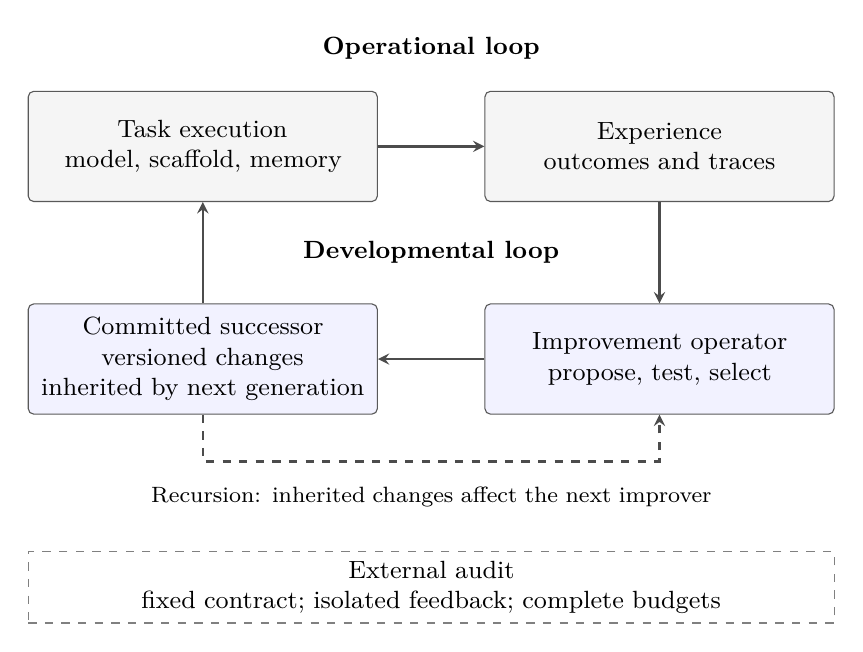
\begin{tikzpicture}[>=stealth, every node/.style={font=\small},
box/.style={draw=black!65, rounded corners=2pt, align=center, minimum height=1.4cm, text width=4.2cm},
arr/.style={->,thick,draw=black!70}]
\node[font=\small\bfseries] at (2.9,1.25) {Operational loop};
\node[box,fill=black!4] (task) at (0,0) {Task execution\\model, scaffold, memory};
\node[box,fill=black!4] (evidence) at (5.8,0) {Experience\\outcomes and traces};
\node[font=\small\bfseries] at (2.9,-1.35) {Developmental loop};
\node[box,fill=blue!5] (improver) at (5.8,-2.7) {Improvement operator\\propose, test, select};
\node[box,fill=blue!5] (commit) at (0,-2.7) {Committed successor\\versioned changes\\inherited by next generation};
\draw[arr] (task)--(evidence);
\draw[arr] (evidence)--(improver);
\draw[arr] (improver)--(commit);
\draw[arr] (commit)--(task);
\draw[arr,dashed] (commit.south) -- (0,-4.0) -- (5.8,-4.0) -- (improver.south);
\node[align=center,text width=10cm,font=\footnotesize] at (2.9,-4.45) {Recursion: inherited changes affect the next improver};
\node[draw=black!50,dashed,align=center,text width=10cm,minimum height=0.85cm] at (2.9,-5.6) {External audit\\fixed contract; isolated feedback; complete budgets};
\end{tikzpicture}
\caption{Two coupled loops and the additional inheritance relation needed for a recursive claim. The external audit is an experimental boundary in the proposed evaluation protocol. This diagram is the survey's synthesis, not a reproduced figure.}
\label{fig:loops}
\end{figure}


An audit evaluator, denoted \(V^*\), is deliberately outside the
modifiable state in the evaluation protocol proposed later. This is an
experimental boundary, not a metaphysical claim that a real system has
an immutable external judge. Internal evaluators may evolve, but their
progress must be assessed against evidence that the candidate cannot
freely redefine.

\hypertarget{three-distinctions-and-a-stronger-hypothesis}{%
\subsection{Three distinctions and a stronger
hypothesis}\label{three-distinctions-and-a-stronger-hypothesis}}

\textbf{Transient refinement} changes an answer, plan, or working
context during an episode without preserving the change for later
episodes. \textbf{Persistent self-improvement} commits a model, memory,
tool, prompt, or code update induced by the system's experience.
\textbf{Recursive improvement} further changes the inherited mechanism
used to generate or select subsequent improvements. These categories
characterize mechanisms; they are not an ordinal safety or intelligence
scale.

An additional claim, \textbf{sustained recursive acceleration}, concerns
the dynamics of a sequence of improvements. It requires evidence that
the capacity to produce useful changes increases over repeated
generations under an explicit treatment of resources and task
difficulty. It does not follow from self-reference alone. A self-editing
program can plateau, oscillate, become more expensive, or destroy
capabilities that matter outside its selection benchmark.

Weight changes are neither necessary nor sufficient for the operational
definition used here. A frozen foundation model combined with a changing
code-based improver can exhibit bounded recursion at the compound-system
level. Conversely, a neural network trained repeatedly by a fixed
optimizer exhibits learning without demonstrating that the optimizer or
the overall improvement mechanism became more effective. STOP uses a
stricter terminology and explicitly avoids claiming full RSI because its
underlying language model remains fixed \citep{stop2023}. Reporting the
boundary resolves much of this apparent disagreement.

Likewise, a system that trains another model is not automatically
improving itself. A successor relation must be specified: does the
resulting model, optimizer, or scaffold become part of the next research
agent? Without this inheritance, the result supports automated AI
development, which is relevant to RSI but does not establish a closed
recursive lineage.

\hypertarget{mechanisms-and-evidence-should-be-reported-separately}{%
\subsection{Mechanisms and evidence should be reported
separately}\label{mechanisms-and-evidence-should-be-reported-separately}}

A useful description records both the proposed modification and the
evidence supporting its effect. We use four evidential questions: does a
benefit survive a fresh session; does it survive a matched resource
comparison; does the updated improver outperform a frozen improver from
comparable starting conditions; and does that advantage survive further
generations or distribution shifts? These are separable questions rather
than mandatory levels of one ladder.

For example, transferring an evolved scaffold to another model supports
portability of the scaffold. It does not by itself show that the
transplanted system is better at producing its next modification.
Similarly, a successful code rewrite demonstrates execution and
persistence; it does not establish that the rewrite caused a gain rather
than merely accompanying additional search. This separation prevents
architectural access from being mistaken for demonstrated capability.

\hypertarget{mechanistic-lineages}{%
\section{Mechanistic lineages}\label{mechanistic-lineages}}

\hypertarget{formal-self-modification-meta-learning-and-open-ended-search}{%
\subsection{Formal self-modification, meta-learning, and open-ended
search}\label{formal-self-modification-meta-learning-and-open-ended-search}}

The Gödel machine is a conceptual anchor because it makes improvement of
the system's own software part of the optimization problem. Its
guarantees are conditional on the axioms, utility specification, and
availability of suitable proofs. They do not guarantee that useful
proofs will be found cheaply or that a specified utility captures all
real-world interests \citep{goedel2003}. An empirical coding agent
inspired by this idea does not inherit the theorem merely by evaluating
a patch with tests.

Learned optimizers provide a different route to improving improvement
procedures. Andrychowicz et al.~learn optimization behavior from a
distribution of training problems, while AutoML-Zero searches over
low-level programmatic building blocks for learning algorithms
\citep{learnoptimizer2016, automlzero2020}. These methods can improve a
learner's update rule without requiring that the learner autonomously
redesign the entire outer search process. They also highlight an older
and still relevant issue: improvement is measured relative to a chosen
task distribution and search representation.

Self-play and environment co-evolution contribute mechanisms for
producing changing learning challenges. AlphaZero's predecessor
formulation learns chess and shogi behavior through self-play under a
fixed game specification and training procedure \citep{alphazero2017}.
POET jointly develops environments and their solutions, with transfer
between evolving tasks \citep{poet2019}. Neither changing opponents nor
increasingly difficult environments alone establishes recursive
algorithm redesign. Their relevance is that useful learning
opportunities can be generated by the system rather than supplied as a
static list.

\hypertarget{output-revision-memory-and-reusable-tools}{%
\subsection{Output revision, memory, and reusable
tools}\label{output-revision-memory-and-reusable-tools}}

Self-Refine uses feedback on a generated output to guide another
revision; Reflexion stores verbal feedback that can influence subsequent
attempts; Voyager accumulates an executable skill library during
exploration \citep{selfrefine2023, reflexion2023, voyager2023}. They
illustrate distinct persistence boundaries. Output refinement can remain
episode-local, whereas retained feedback and skills can change later
behavior without updating model weights. Toolformer adds a parametric
route by training a model on automatically selected tool-use examples
\citep{toolformer2023}.

These methods matter to RSI because a reliable improver needs memory,
tools, and error correction. However, adding an experience to memory is
only a candidate mechanism. A fresh-session comparison must show that it
is retrieved and used appropriately, and that stale or irrelevant
experience does not impair later tasks. The stronger question is whether
the system improves how it writes, selects, retrieves, or revises that
memory.

Intrinsic self-correction also has a contested empirical record. Huang
et al.~find failures of reasoning self-correction without external
feedback in their studied settings, whereas subsequent work reports that
prompt fairness and decoding choices materially affect the outcome
\citep{intrinsic2023, intrinsicpositive2024}. SCoRe trains multi-turn
self-correction through reinforcement learning and reports improvements
after targeted training \citep{score2024}. These findings concern
different interventions. They do not warrant either a universal
impossibility claim or an assumption that repeated untrained
self-critique is reliably beneficial.

\hypertarget{synthetic-supervision-and-co-evolving-curricula}{%
\subsection{Synthetic supervision and co-evolving
curricula}\label{synthetic-supervision-and-co-evolving-curricula}}

STaR bootstraps reasoning traces into further training, while
Self-Instruct generates and filters instruction-following examples
\citep{star2022, selfinstruct2022}. Such pipelines can consolidate
useful behavior into parameters. They do not create information from
nothing: pretrained knowledge, seed examples, filtering rules, known
answers, and environmental regularities can all contribute supervision.
A training dataset's origin should therefore be described component by
component rather than compressed into ``self-generated.''

Self-Rewarding Language Models couples response generation and
model-produced evaluative feedback across iterative preference
optimization. SPIN instead learns through a self-play objective anchored
in a supervised dataset \citep{selfreward2024, spin2024}. Their feedback
channels differ. A model-generated preference is a learned judgment; a
supervised reference is an external anchor relative to the generated
alternative. Neither channel should automatically be treated as
error-free.

Reinforcement learning with verifiable rewards offers another path.
DeepSeek-R1 demonstrates that reinforcement learning can substantially
shape reasoning behavior, but its training procedures are not thereby
autonomously self-redesigned \citep{r12025}. Absolute Zero Reasoner
(AZR) couples task proposal and solving through executable code-based
feedback \citep{azr2025}. R-Zero co-evolves challenger and solver models
and derives pseudo-labels through the solver's answer agreement
\citep{rzero2025}. Executable verification and majority agreement have
different error properties: a consensus answer can be systematically
wrong, while a passing execution check can still cover only a limited
specification.

``Zero data'' in these studies refers to a particular post-training
input regime. It does not mean absence of pretraining, human-authored
software, chosen objectives, or environmental structure. Their main
importance is to redistribute curriculum and supervision work from a
fixed human-curated post-training dataset into an automated loop.
Whether that loop improves its own learning mechanism remains a separate
empirical question.

\hypertarget{evolving-prompts-scaffolds-and-improvers}{%
\subsection{Evolving prompts, scaffolds, and
improvers}\label{evolving-prompts-scaffolds-and-improvers}}

Automated Design of Agentic Systems (ADAS) uses a meta-agent to program
candidate agents and maintains an archive of prior designs. GEPA uses
natural-language reflection and evolutionary selection to optimize
prompts \citep{adas2024, gepa2025}. Both make substantial parts of agent
construction searchable. Yet optimizing a prompt or an agent
architecture with a fixed search controller is different from modifying
the controller that performs the search.

STOP directly applies an improver program to itself. The resulting
program changes how language-model calls are organized to improve
downstream programs \citep{stop2023}. Gödel Agent likewise exposes the
agent's logic to self-directed modification \citep{goedelagent2024}.
These systems move the object of search toward the developmental
mechanism. The remaining external structure, including objectives,
runtime limits, model APIs, and evaluation procedures, still matters
when interpreting how much of the loop has closed.

SICA and Darwin Gödel Machine (DGM) make self-modification concrete in
coding agents. DGM retains a population archive that allows previously
discovered agents to seed further changes; SICA optimizes an agent
through its own coding capabilities \citep{sica2025, dgm2025}. Their
results support the value of inherited scaffolds, but the empirical
interpretation depends on subsets, budgets, selection, and controls. In
DGM's consulted version, archive maintenance and parent selection remain
fixed. The boundary therefore includes an evolving self-modifying agent
within an externally specified evolutionary process.

HGM targets a weakness of selecting parents by present task performance.
It estimates clade-level metaproductivity from descendant outcomes and
separates expansion, evaluation, and selection decisions
\citep{hgm2025}. This is directly relevant to the question ``does the
improver improve?'' However, a proposed outer search strategy should not
automatically be described as autonomously discovered. Its evidential
contribution concerns lineage-sensitive search and reported comparisons,
not elimination of all human-designed improvement machinery.

\hypertarget{self-directed-weight-adaptation}{%
\subsection{Self-directed weight
adaptation}\label{self-directed-weight-adaptation}}

SEAL trains a model to generate self-edits: training data and update
directives whose utility is assessed after adaptation. Its outer
reinforcement-learning loop rewards edits that improve the adapted
model's downstream performance \citep{seal2025}. This gives the language
model a role in choosing how new information becomes a parameter update.
It also illustrates why persistence requires careful qualification: an
adaptation episode, a deployed accumulated model, and an outer-loop
training run are different objects.

Search over Self-Edit Strategies studies a narrower extension in which
the model searches over adaptation templates and selected
hyperparameters. Its reported setup uses one round of self-improvement;
an archive helps relative to a weaker template but does not surpass the
strongest human-designed baseline, and homogenization remains a concern
\citep{selfedit2026}. This is useful negative or limiting evidence.
Enlarging a modifiable interface does not guarantee that the model
exploits the added freedom productively.

A full evaluation should distinguish improvement of edit proposals from
improvement caused by a stronger starting model or a different training
budget. It should also measure whether previous adaptations are
retained. A system that incorporates new information efficiently while
repeatedly damaging old capabilities has not demonstrated an
unrestricted cumulative learning process.

\hypertarget{algorithm-discovery-and-automated-research}{%
\subsection{Algorithm discovery and automated
research}\label{algorithm-discovery-and-automated-research}}

FunSearch combines pretrained language-model proposals, program
evaluation, and a population of candidates to discover useful programs.
AlphaEvolve extends evolutionary coding to a broader set of algorithmic
and infrastructure problems \citep{funsearch2024, alphaevolve2025}.
These systems show why external execution can make a generative model
useful beyond its unaided responses. Improving infrastructure used in
model development creates a potentially important feedback path, but
that path should be measured end to end before it is called autonomous
recursive acceleration.

The AI Scientist and its successor automate portions of hypothesis
generation, experimentation, analysis, and manuscript preparation
\citep{scientist2024, scientistv22025}. A completed paper or successful
experiment is evidence of research automation. For RSI, the critical
additional step is inheritance: does the discovery improve the
researcher that will conduct the next research cycle? Scientific output
volume, reviewer scores, and successor-model capability are not
interchangeable measures.

The field therefore contains several partially connected loops. An
improved coding scaffold can build a better data generator; the
generator can improve a model; the model can propose better scaffold
changes. Such coupling is plausible, but a diagram of the coupling is
not evidence that its net gain is positive. Interface costs, transfer
losses, evaluation noise, and model-training expense may dominate the
apparent local improvements.

\hypertarget{comparative-evidence-from-representative-systems}{%
\section{Comparative evidence from representative
systems}\label{comparative-evidence-from-representative-systems}}

Table \ref{tab:mechanisms} summarizes mechanism boundaries. ``Recursive
relevance'' denotes our interpretation of the described design, not an
independently verified grade.

\begin{longtable}{p{0.16\linewidth}p{0.22\linewidth}p{0.23\linewidth}p{0.29\linewidth}}
\caption{Representative mechanisms and the boundary of recursive claims.}\label{tab:mechanisms}\\
\toprule
Family & Persistent object & Main feedback & Recursive relevance and boundary \\
\midrule\endfirsthead
\toprule Family & Persistent object & Main feedback & Recursive relevance and boundary \\
\midrule\endhead
Self-Refine & Usually episode-local output & Model critique & Refinement unless changes are retained. \\
Reflexion / Voyager & Memory / executable skills & Task and environment feedback & Persistent adaptation; update mechanism need not evolve. \\
STaR / Self-Instruct & Model parameters & Filtered synthetic supervision & Self-training within a specified pipeline. \\
Self-Rewarding & Policy and judging behavior & Learned preferences & Coupled improvement claims require external calibration. \\
AZR / R-Zero & Policy and curriculum & Execution / answer consensus & Adaptive curriculum; grounding differs substantially. \\
ADAS / GEPA & Agent code / prompts & Task evaluations and traces & Design automation with an outer search procedure. \\
STOP / G\"odel Agent & Improver or agent logic & Downstream utility & Direct bounded self-reference; resources and judge remain specified. \\
SICA / DGM & Self-modifying scaffold & Coding benchmarks & Inherited code changes; base models and some outer logic remain fixed. \\
HGM & Descendant population & Lineage-based estimates & Measures productive ancestry; outer search is an authored method. \\
SEAL & Self-edit policy and adapted weights & Post-update task performance & Learns adaptation choices inside a prescribed outer loop. \\
FunSearch / AlphaEvolve & Candidate programs & Executable evaluators & Discovery can aid AI development; inheritance must be demonstrated. \\
AI Scientist & Research artifacts & Experiments and review & Research automation; successor feedback is an additional claim. \\
\bottomrule
\end{longtable}

Several numerical examples show why the evaluation unit matters. DGM
reports an increase from 20.0\% to 50.0\% on its SWE-bench evaluation
subset and from 14.2\% to 30.7\% on the full Polyglot benchmark. Its
SWE-bench results should not be presented as a score on the full
official suite. The paper also includes frozen-improver and archive
ablations, which are more informative for recursive claims than endpoint
scores alone \citep{dgm2025}.

SICA reports 17\% to 53\% on a random SWE-bench Verified subset. Its
experiment combines a 50-question SWE-bench subset with other tasks,
includes time and monetary cost in the utility, and reports
approximately US\$7,000 in API cost for a 15-iteration run
\citep{sica2025}. These qualifications identify a bounded experiment,
not a general deployment-wide rate of improvement. The SICA and DGM
percentages should not be ranked against each other because their
evaluation configurations differ.

HGM's comparison explicitly investigates descendant productivity rather
than treating present performance as a sufficient proxy \citep{hgm2025}.
This supports a shift toward measuring the developmental process.
Nevertheless, transfer of a discovered scaffold, prediction of
productive lineages, and causal improvement of a reusable operator
remain distinguishable results. The proposed protocol in the next
section is intended to help separate them without discounting their
practical value.

The emerging 2026 benchmarks add complementary measurement targets.
PAST-Bench compares later fresh-session behavior with access to retained
experience enabled or disabled, and examines evidence of the persistence
pathway \citep{pastbench2026}. RSIBench-Data fixes the surrounding
post-training stack while agents revise training-data strategies. It
reports improvement over the first valid attempt in 58.33\% of settings;
among searches continuing after their observed peak, 78.26\% finish
below that peak \citep{rsidata2026}. The latter statistic describes
regression relative to the within-run maximum in a selected set of runs.
It is not the probability that one additional research iteration harms a
randomly chosen system.

PostTrainBench allows agents to undertake post-training within a bounded
GPU budget and documents both successful targeted adaptation and
failures involving benchmark or resource boundaries
\citep{posttrain2026}. AI4AI-Bench separates an agent's four-hour
development period from a subsequent clean-start run of up to twelve
hours, using a hidden final evaluator across ten research repositories
\citep{ai4ai2026}. These benchmarks make parts of the AI-development
process testable. Neither a data-research benchmark nor an
algorithm-design benchmark, by itself, establishes that the trained
successor repeatedly becomes a better researcher.

\hypertarget{evaluating-the-capacity-to-improve}{%
\section{Evaluating the capacity to
improve}\label{evaluating-the-capacity-to-improve}}

\hypertarget{what-existing-benchmarks-measure}{%
\subsection{What existing benchmarks
measure}\label{what-existing-benchmarks-measure}}

SWE-bench measures repository-level issue resolution; MLE-bench measures
machine-learning engineering; RE-Bench examines research-engineering
performance with comparisons to human experts
\citep{swebench2023, mlebench2024, rebench2024}. They can serve as
useful operational outcomes, yet a single score on any of them is not an
intrinsic measure of recursive improvement. A benchmark that tests the
products of research may never test the next researcher's ability to
improve them further.

PAST-Bench addresses experience retention, RSIBench-Data addresses
training-data decisions, PostTrainBench addresses autonomous
post-training, and AI4AI-Bench emphasizes algorithmic changes
\citep{pastbench2026, rsidata2026, posttrain2026, ai4ai2026}. Together
they motivate a modular evaluation suite rather than one universal RSI
number. The relevant modules are persistence, productive proposal, valid
selection, inheritance, and multi-generation transfer.

\hypertarget{a-matched-operator-comparison}{%
\subsection{A matched-operator
comparison}\label{a-matched-operator-comparison}}

To evaluate an improver, let \(A\) be a starting target system, \(U\) an
improvement operator, \(b\) a development budget, and \(V^*\) an
isolated audit evaluator. Define a proposed measure of
\textbf{improvement yield}:

\[
Y(U,A;b)=\mathbb{E}\left[V^*(\operatorname{Run}(U,A;b))-V^*(A)\right].
\]

The expectation is over task draws and relevant randomness. Audit
inference budgets and environment versions are fixed separately. An
updated operator \(U_t\) can then be compared with a baseline operator
\(U_0\) on the same distribution of starting systems:

\[
\Delta_{\mathrm{op}}(b)=\mathbb{E}_{A\sim\mathcal{A}_{\mathrm{audit}}}
\left[Y(U_t,A;b)-Y(U_0,A;b)\right].
\]

A positive estimate supports an operator advantage in the specified
setting. It does not establish universal superiority. Matching \(A\)
matters because a newer operator may otherwise be evaluated only on a
more capable target, or on a target with different remaining headroom.
Likewise, the operator's development cost must be charged when comparing
complete methods: conditional reuse of an already learned operator and
end-to-end discovery of that operator answer different economic
questions.

The comparison is a synthesis of existing concerns about
metaproductivity, controlled persistence, and adaptive data analysis
\citep{hgm2025, pastbench2026, adaptive2015}. It is not a new theorem,
and we have not demonstrated that this particular measure predicts
long-run general progress.

\hypertarget{factorial-controls-and-coupled-systems}{%
\subsection{Factorial controls and coupled
systems}\label{factorial-controls-and-coupled-systems}}

When the target and improver can be separated, a two-by-two experiment
helps distinguish their contributions:

\begin{longtable}[]{@{}lll@{}}
\toprule
\begin{minipage}[b]{0.30\columnwidth}\raggedright
Starting target\strut
\end{minipage} & \begin{minipage}[b]{0.30\columnwidth}\raggedright
Original operator \(U_0\)\strut
\end{minipage} & \begin{minipage}[b]{0.30\columnwidth}\raggedright
Updated operator \(U_t\)\strut
\end{minipage}\tabularnewline
\midrule
\endhead
\begin{minipage}[t]{0.30\columnwidth}\raggedright
Original target \(A_0\)\strut
\end{minipage} & \begin{minipage}[t]{0.30\columnwidth}\raggedright
Baseline development run\strut
\end{minipage} & \begin{minipage}[t]{0.30\columnwidth}\raggedright
Operator effect from the original target\strut
\end{minipage}\tabularnewline
\begin{minipage}[t]{0.30\columnwidth}\raggedright
Updated target \(A_t\)\strut
\end{minipage} & \begin{minipage}[t]{0.30\columnwidth}\raggedright
Target-state effect under fixed improvement\strut
\end{minipage} & \begin{minipage}[t]{0.30\columnwidth}\raggedright
Joint effect and possible interaction\strut
\end{minipage}\tabularnewline
\bottomrule
\end{longtable}

Every cell uses the same declared development budget, audit protocol,
and task split. Comparing columns within a row estimates an operator
effect conditional on that target. Comparing rows changes both
capability and headroom, so it requires more caution. The factorial
design also reveals whether a new operator works only with its own
evolved target.

Some systems are tightly coupled: changing the model changes both the
solver and the improver, and no clean transplant preserves
functionality. In that case, forcing a decomposition would create an
artificial system. Researchers should instead compare full lineages
against frozen-update controls, identify the intervention precisely, and
report the unresolved attribution. Functional self-reference is a
property of a system; experimentally isolating its causal contribution
is an additional challenge.

Useful controls include a frozen improver given an equal
candidate-generation budget, a replay or random-search controller with
the same evaluation budget, and a no-persistence condition that removes
learned state without changing the task prompt. Equal inference-time
sampling is especially important: an evolved agent that simply makes
more model calls may improve raw accuracy without improving efficiency.
Such a result is still useful, but the claimed resource tradeoff should
be explicit.

\hypertarget{separating-development-feedback-from-audit-evidence}{%
\subsection{Separating development feedback from audit
evidence}\label{separating-development-feedback-from-audit-evidence}}

A robust protocol distinguishes development tasks, selection feedback,
and final audit tasks. Candidate search can repeatedly inspect
development feedback. Selection procedures can use a separately
specified budget of validation feedback. The final audit should assess a
frozen candidate or frozen lineage without returning task-specific
information that guides further selection. Repeatedly consulting a
supposed holdout makes it part of an adaptive optimization process
\citep{adaptive2015}.

For long-running systems, one untouched holdout is not enough forever.
Successive external audits need fresh task families, controlled
disclosure, or a statistical procedure explicitly designed for adaptive
reuse. Secret tests reduce direct memorization but do not automatically
ensure construct validity. EvalPlus shows the importance of stronger
test coverage for evaluating generated code; similarly, an RSI evaluator
must check whether the test captures the claimed improvement rather than
merely a convenient proxy \citep{evalplus2023}.

Operator transfer deserves its own split. If an improver is developed on
one group of codebases, it should be tested on new starting agents or
repositories and, where relevant, on another model family. A stronger
test asks whether the transplanted improver can generate useful
descendants in the new setting. Testing only the transferred agent's
immediate task performance answers a weaker question.

\hypertarget{lineages-selection-and-statistical-uncertainty}{%
\subsection{Lineages, selection, and statistical
uncertainty}\label{lineages-selection-and-statistical-uncertainty}}

A self-improvement experiment should retain the entire ancestry graph:
candidate hashes, parent identifiers, proposed edits, evaluation access,
rejected changes, crashes, and selection decisions. The lineage is the
unit that reveals how a modification affected future possibilities.
Reporting only the final best agent erases failed branches and makes it
difficult to distinguish a productive research procedure from an
unusually fortunate draw.

Three curves should be separated: the current deployed candidate, the
best candidate selected using permitted validation information, and the
retrospective best under audit scores. The last is an analysis artifact,
not a deployable selection policy, unless the audit information was
available by design and charged to development. A best-so-far curve is
non-decreasing by construction; it does not demonstrate that successive
modifications are reliably beneficial.

Uncertainty should reflect the level at which treatment was assigned.
Task outcomes within one evolved lineage share ancestry and selection
history, so treating them as fully independent repetitions can
exaggerate precision. Independent lineages, task-family resampling, and
paired evaluations with common random seeds address different variance
sources. Reports should disclose the number of independent runs and the
method used for confidence intervals, rather than assigning a universal
sufficient number of seeds.

\hypertarget{costs-persistence-and-acceleration}{%
\subsection{Costs, persistence, and
acceleration}\label{costs-persistence-and-acceleration}}

Resource accounting should include proposal-model inference, candidate
execution, evaluator calls, model updates, rejected runs, storage or
retrieval overhead where material, and human interventions. Wall time,
API expenditure, GPU-hours, and inference tokens are different
quantities. A method can improve wall time through parallelism while
increasing total compute. A paper should report the relevant vector of
costs instead of treating one convenient scalar as a universal budget.

Persistence is measured by evaluating a committed system in fresh
sessions without replaying privileged development traces. Capability
retention requires additional tests on previous tasks and constraints.
These tests prevent a narrow optimization from being described as
cumulative progress when it simply trades one capability for another. If
a system changes its goals, comparisons under a stable external
objective should be retained; a self-chosen easier objective does not
constitute improvement on the original objective.

To study acceleration, let \(C_t\) be cumulative development cost and
\(P_t\) an externally measured performance value on a stable or
explicitly calibrated task distribution. A simple descriptive increment
is

\[
 g_t=\frac{P_{t+1}-P_t}{C_{t+1}-C_t}.
\]

An increase in \(g_t\) over a few observations is not proof of
persistent acceleration. The pattern may reflect noise, headroom,
changed task difficulty, or a favorable branch. A stronger claim
requires replicated generations, an appropriate fixed-improver
counterfactual, explicit treatment of changing resources, and transfer
beyond the selected benchmark. Saturating scores also make this ratio
hard to interpret. We therefore recommend reporting cost--performance
frontiers and operator-yield curves together with raw trajectories,
without extrapolating a finite experiment into an intelligence-explosion
forecast.

\hypertarget{failure-modes-and-safety-boundaries}{%
\section{Failure modes and safety
boundaries}\label{failure-modes-and-safety-boundaries}}

\hypertarget{feedback-quality-and-evaluator-co-adaptation}{%
\subsection{Feedback quality and evaluator
co-adaptation}\label{feedback-quality-and-evaluator-co-adaptation}}

No improvement loop can be interpreted independently of its feedback.
LLM judges exhibit biases and limitations documented in benchmark
evaluation, while optimizing a proxy reward can reduce performance under
a separate reference measure \citep{judge2023, rewardoveropt2022}. If a
proposer and its evaluator share blind spots, repeated agreement can
increase apparent confidence without supplying independent evidence of
correctness.

This does not establish a universal ordering in which every formal check
is better than every human or model judgment. A proof is strong evidence
for the formal proposition it proves; the proposition can still omit an
important requirement. A compiler checks a narrower property than a
comprehensive behavioral test. A domain expert can evaluate concerns not
represented in either. The appropriate question is which failure modes
the signal detects, at what cost, and with what calibration to the
desired outcome.

When the evaluator itself changes, a further identification problem
arises. A higher score can result from a more capable candidate, a more
permissive judge, or a changed objective. Evaluate new judges against
independently labeled or executable cases, including adversarial
disagreement cases, and preserve a reference evaluation that the
candidate cannot rewrite. Calibration performance should be reported
separately from the policy's score under the new judge.

\hypertarget{collapse-forgetting-and-loss-of-diversity}{%
\subsection{Collapse, forgetting, and loss of
diversity}\label{collapse-forgetting-and-loss-of-diversity}}

Recursive training on model-generated data can lose information about
the original data distribution. The model-collapse literature
demonstrates this risk under particular training and sampling
conditions; work on accumulating real and synthetic data shows that
collapse is not an inevitable consequence of any synthetic-data use
\citep{collapse2023, accumulate2024}. The conclusion is conditional:
replacement, accumulation, filtering, and grounding produce different
dynamics.

In agent evolution, diversity can disappear even without parameter
training. Candidate programs can converge on similar prompts,
architectures, or habits because the generator repeatedly conditions on
the same successful examples. Self-edit search provides a concrete
report of homogenization concerns \citep{selfedit2026}. Archives can
preserve alternatives, but textual variety is not the same as behavioral
diversity. Evaluation should probe distinct strategies and transfer
properties, as well as the number of stored candidates.

Forgetting presents another tradeoff. A change that improves coding
speed can damage error recovery; a memory consolidation rule can discard
rare but important constraints. Retention and regression tests should
therefore be part of acceptance rather than deferred until deployment.
Maintaining a recoverable previous version limits operational damage but
does not, by itself, make the research process reliably progressive.

\hypertarget{self-modification-and-control-integrity}{%
\subsection{Self-modification and control
integrity}\label{self-modification-and-control-integrity}}

If an agent can edit its evaluator, permissions, logs, or budget
accounting, it can alter the measurement and control system as well as
the intended task solution. Reward-tampering research provides a causal
framework for analyzing such incentives, and PostTrainBench documents
relevant boundary violations in contemporary automated training
experiments \citep{tampering2019, posttrain2026}. These are concrete
reasons to distinguish the modifiable research workspace from the
externally enforced evaluation and resource boundary.

For research systems, a defensible default is to version candidate code
and models, isolate execution, restrict access to audit assets and
credentials, enforce budgets outside candidate code, and preserve
rollback artifacts. More capable internal evaluation can still evolve
within this arrangement. The restriction protects the interpretation of
the experiment as well as the environment in which it runs.

Broader loss-of-control scenarios remain important hypotheses, but the
reviewed bounded experiments do not determine their likelihood or
timescale. Conversely, failure to demonstrate open-ended acceleration is
not evidence that self-modifying systems are harmless. Scientific claims
about recursive capability and engineering decisions about containment
should use the evidence appropriate to each question.

\hypertarget{research-priorities}{%
\section{Research priorities}\label{research-priorities}}

\textbf{Measure inheritance directly.} Automated AI research should
report what artifact is inherited by the next researcher, how it is
integrated, and whether it improves subsequent research yield. This
would connect training-algorithm and data-research benchmarks to
multi-generation RSI experiments rather than treating successful
training as closure of the loop.

\textbf{Develop transferable improver tests.} Benchmarks should separate
the tasks used to learn an improver from the target systems on which it
is asked to make new improvements. Transfer should include producing
useful descendants, not only solving new tasks with an already evolved
agent. Coupled-system cases need carefully specified lineage controls
when transplantation is impossible.

\textbf{Learn evaluation without surrendering measurement.}
Self-rewarding and evaluator adaptation are attractive because external
labels are expensive. Research should test whether a new evaluator
detects errors missed by the previous one, including errors the
generator is incentivized to exploit. A growing evaluation capability
and a fixed audit contract can coexist.

\textbf{Report the economics of improvement.} Local speedups in coding,
training kernels, or data preparation should be related to total
development cost. An expensive improver may be worthwhile when reused
widely, but its amortization assumptions must be explicit. A gain in one
infrastructure component need not translate proportionally into faster
overall research.

\textbf{Study long-horizon regressions and branching.} Strong
checkpoints can appear early, and later changes may fail to surpass
them. Research should compare lineage selection, checkpoint
preservation, diversity maintenance, and stopping rules. Rejected
proposals are useful data about the search process and should not
disappear from public evidence.

\textbf{Create shared reporting artifacts.} A minimum reproducibility
record should include system boundaries, candidate and parent versions,
model identifiers, task splits, evaluator access, complete budgets,
selection rules, independent-run counts, and failure logs. These
artifacts would permit more meaningful comparisons even when full model
weights or proprietary APIs cannot be released.

\hypertarget{limitations-of-this-survey}{%
\section{Limitations of this survey}\label{limitations-of-this-survey}}

The selection is weighted toward language models, coding agents, and
computational research because these areas provide inspectable artifacts
and executable feedback. Robotics, hardware self-design, developmental
learning, and older evolutionary-computation literature are not
comprehensively covered. The reference set is a curated sample, and
conclusions about the absence of stronger evidence are restricted to
that sample rather than asserted as a proof of global absence.

Several central sources are preprints, and some claims depend on
proprietary models or author-run infrastructure. Metadata checks do not
establish result validity. Differences in task subsets, model versions,
budgets, and evaluation access prevent a reliable cross-paper
effect-size aggregation. Our proposed operator-yield comparisons also
require experimental validation, especially for coupled agents and
changing task distributions. No new benchmark results, independent
replications, or forecasts are presented.

\hypertarget{conclusion}{%
\section{Conclusion}\label{conclusion}}

RSI is best studied as an explicit relationship between inherited system
changes and the process that generates further changes. Existing work
provides important mechanisms for persistent learning, self-directed
adaptation, self-modifying scaffolds, productive lineage search, and
automated AI research. In the selected literature, these mechanisms
support bounded forms of self-improvement, while general, sustained,
resource-normalized recursive acceleration remains unestablished.

The next empirical step is to connect mechanism, inheritance, and
measurement. Matched improver comparisons, isolated audit feedback,
complete lineage records, and honest cost accounting can show when an
improvement procedure itself becomes more effective. These practices
would make both positive results and plateaus scientifically
informative, and reduce the distance between evocative claims of
automatic evolution and reproducible evidence.

\hypertarget{transparency-statement}{%
\section{Transparency statement}\label{transparency-statement}}

AI assisted retrieval, drafting, translation, and typesetting. No new
experiments were conducted. The source register and evidence ledger
document the synthesis; the proposed evaluation protocol remains
unvalidated.

\clearpage
\appendix

\hypertarget{a-compact-reporting-template}{%
\section{A compact reporting
template}\label{a-compact-reporting-template}}

\begin{longtable}[]{@{}ll@{}}
\toprule
\begin{minipage}[b]{0.47\columnwidth}\raggedright
Item\strut
\end{minipage} & \begin{minipage}[b]{0.47\columnwidth}\raggedright
Information needed to interpret an RSI claim\strut
\end{minipage}\tabularnewline
\midrule
\endhead
\begin{minipage}[t]{0.47\columnwidth}\raggedright
System boundary\strut
\end{minipage} & \begin{minipage}[t]{0.47\columnwidth}\raggedright
Model, scaffold, memory, data, improver, evaluator; mutable and
externally fixed components\strut
\end{minipage}\tabularnewline
\begin{minipage}[t]{0.47\columnwidth}\raggedright
Claimed mechanism\strut
\end{minipage} & \begin{minipage}[t]{0.47\columnwidth}\raggedright
Refinement, persistent adaptation, operator improvement, or repeated
acceleration\strut
\end{minipage}\tabularnewline
\begin{minipage}[t]{0.47\columnwidth}\raggedright
Inheritance\strut
\end{minipage} & \begin{minipage}[t]{0.47\columnwidth}\raggedright
Exact artifact passed to the next generation; whether the successor
conducts the next improvement\strut
\end{minipage}\tabularnewline
\begin{minipage}[t]{0.47\columnwidth}\raggedright
Controls\strut
\end{minipage} & \begin{minipage}[t]{0.47\columnwidth}\raggedright
Frozen improver, matched starting target, no persistence, equivalent
search and inference budgets\strut
\end{minipage}\tabularnewline
\begin{minipage}[t]{0.47\columnwidth}\raggedright
Evaluation access\strut
\end{minipage} & \begin{minipage}[t]{0.47\columnwidth}\raggedright
Development, selection, and audit tasks; feedback returned at each
stage\strut
\end{minipage}\tabularnewline
\begin{minipage}[t]{0.47\columnwidth}\raggedright
Selection\strut
\end{minipage} & \begin{minipage}[t]{0.47\columnwidth}\raggedright
Current, validation-selected, and retrospective-best candidates reported
separately\strut
\end{minipage}\tabularnewline
\begin{minipage}[t]{0.47\columnwidth}\raggedright
Resources\strut
\end{minipage} & \begin{minipage}[t]{0.47\columnwidth}\raggedright
Proposal, evaluation, training, failed runs, human work, and deployment
inference\strut
\end{minipage}\tabularnewline
\begin{minipage}[t]{0.47\columnwidth}\raggedright
Uncertainty\strut
\end{minipage} & \begin{minipage}[t]{0.47\columnwidth}\raggedright
Independent lineages, task-family variation, paired design,
confidence-interval method\strut
\end{minipage}\tabularnewline
\begin{minipage}[t]{0.47\columnwidth}\raggedright
Transfer and retention\strut
\end{minipage} & \begin{minipage}[t]{0.47\columnwidth}\raggedright
New targets and model families; subsequent improvement; old capability
regressions\strut
\end{minipage}\tabularnewline
\begin{minipage}[t]{0.47\columnwidth}\raggedright
Reproducibility\strut
\end{minipage} & \begin{minipage}[t]{0.47\columnwidth}\raggedright
Versioned artifacts, ancestry graph, logs, seeds, model identifiers, and
failure cases\strut
\end{minipage}\tabularnewline
\bottomrule
\end{longtable}

\Needspace{15\baselineskip}

\hypertarget{operational-glossary}{%
\section{Operational glossary}\label{operational-glossary}}

\begin{longtable}[]{@{}ll@{}}
\toprule
\begin{minipage}[b]{0.47\columnwidth}\raggedright
Term\strut
\end{minipage} & \begin{minipage}[b]{0.47\columnwidth}\raggedright
Meaning in this survey\strut
\end{minipage}\tabularnewline
\midrule
\endhead
\begin{minipage}[t]{0.47\columnwidth}\raggedright
Recursive self-improvement\strut
\end{minipage} & \begin{minipage}[t]{0.47\columnwidth}\raggedright
Inherited change to a mechanism used for subsequent improvement\strut
\end{minipage}\tabularnewline
\begin{minipage}[t]{0.47\columnwidth}\raggedright
Persistent adaptation\strut
\end{minipage} & \begin{minipage}[t]{0.47\columnwidth}\raggedright
A committed change available beyond the original episode\strut
\end{minipage}\tabularnewline
\begin{minipage}[t]{0.47\columnwidth}\raggedright
Improvement operator\strut
\end{minipage} & \begin{minipage}[t]{0.47\columnwidth}\raggedright
The procedure that proposes or selects changes to a target system\strut
\end{minipage}\tabularnewline
\begin{minipage}[t]{0.47\columnwidth}\raggedright
Agent scaffold or harness\strut
\end{minipage} & \begin{minipage}[t]{0.47\columnwidth}\raggedright
Prompts, tools, memory interfaces, and control flow around a foundation
model\strut
\end{minipage}\tabularnewline
\begin{minipage}[t]{0.47\columnwidth}\raggedright
Metaproductivity\strut
\end{minipage} & \begin{minipage}[t]{0.47\columnwidth}\raggedright
Capacity to produce useful descendants; interpreted relative to a task
and resource setting\strut
\end{minipage}\tabularnewline
\begin{minipage}[t]{0.47\columnwidth}\raggedright
Audit evaluator\strut
\end{minipage} & \begin{minipage}[t]{0.47\columnwidth}\raggedright
An evaluation channel isolated from the candidate's modification and
selection process\strut
\end{minipage}\tabularnewline
\begin{minipage}[t]{0.47\columnwidth}\raggedright
Grounding\strut
\end{minipage} & \begin{minipage}[t]{0.47\columnwidth}\raggedright
Evidence or constraints supplied by an environment, specification, or
independent reference\strut
\end{minipage}\tabularnewline
\bottomrule
\end{longtable}

\clearpage
\bibliography{references.bib}

\end{document}
